



\documentclass[conference]{IEEEtran}



% *** GRAPHICS RELATED PACKAGES ***
%
\ifCLASSINFOpdf
   \usepackage[pdftex]{graphicx}
   %declare the path(s) where your graphic files are
   \graphicspath{{../img/}}
  % and their extensions so you won't have to specify these with
  % every instance of \includegraphics
   \DeclareGraphicsExtensions{.pdf,.jpeg,.png}
\else
  % or other class option (dvipsone, dvipdf, if not using dvips). graphicx
  % will default to the driver specified in the system graphics.cfg if no
  % driver is specified.
  % \usepackage[dvips]{graphicx}
  % declare the path(s) where your graphic files are
  % \graphicspath{{../eps/}}
  % and their extensions so you won't have to specify these with
  % every instance of \includegraphics
  % \DeclareGraphicsExtensions{.eps}
\fi
% graphicx was written by David Carlisle and Sebastian Rahtz. It is
% required if you want graphics, photos, etc. graphicx.sty is already
% installed on most LaTeX systems. The latest version and documentation
% can be obtained at: 
% http://www.ctan.org/pkg/graphicx
% Another good source of documentation is "Using Imported Graphics in
% LaTeX2e" by Keith Reckdahl which can be found at:
% http://www.ctan.org/pkg/epslatex
%
% latex, and pdflatex in dvi mode, support graphics in encapsulated
% postscript (.eps) format. pdflatex in pdf mode supports graphics
% in .pdf, .jpeg, .png and .mps (metapost) formats. Users should ensure
% that all non-photo figures use a vector format (.eps, .pdf, .mps) and
% not a bitmapped formats (.jpeg, .png). The IEEE frowns on bitmapped formats
% which can result in "jaggedy"/blurry rendering of lines and letters as
% well as large increases in file sizes.
%
% You can find documentation about the pdfTeX application at:
% http://www.tug.org/applications/pdftex


\usepackage{url}
\usepackage[table,xcdraw]{xcolor}
\usepackage{eurosym}
\usepackage{amsfonts}
\usepackage{balance}
\usepackage{cite} %this package is awesome - it reorders lists of citations to be in numeric order
\usepackage{pifont}
\usepackage{eqparbox}

% Tables
\usepackage{booktabs}
\usepackage{pbox}
\renewcommand{\arraystretch}{1.2} 
\usepackage{arydshln}
%\renewcommand*\cmidrule{} % No middle lines
%\renewcommand{\arraystretch}{1.5} % Additional spacing with no middle lines
%\renewcommand*\cmidrule{\hdashline[1pt/2pt]}% Dashed middle lines
\renewcommand*\cmidrule{\midrule[0.001em]} % Thin middle lines
%\renewcommand*\cmidrule{\midrule} % Thick middle lines


% correct bad hyphenation here
\hyphenation{op-tical net-works semi-conduc-tor}

\clubpenalty = 10000
\widowpenalty = 10000
\displaywidowpenalty = 10000

\newcommand{\ms}{LEGO MINDSTORMS EV3}
\newcommand{\mbs}{\textsc{my blocks}}
\newcommand{\mb}{\textsc{my block}}
\newcommand{\horiz}{\hspace{2.1pt}}
\renewcommand{\topfraction}{.9}
\newcommand{\todo}[1]{\textbf{#1}}

\begin{document}

\title{Code Smells in Education Programming Languages \large{\\Case studies on \ms~and Kodu}}


% author names and affiliations
% use a multiple column layout for up to three different
% affiliations
\author{
\IEEEauthorblockN{Felienne Hermans}
\IEEEauthorblockA{Delft University of Technology\\
Mekelweg 4\\
Delft, the Netherlands\\
f.f.j.hermans@tudelft.nl }
\and
\IEEEauthorblockN{Kathryn T. Stolee}
\IEEEauthorblockA{North Carolina State University\\
Raleigh, NC, USA\\
ktstolee@ncsu.edu}
\and
\IEEEauthorblockN{David Hoepelman}
\IEEEauthorblockA{Delft University of Technology\\
Mekelweg 4\\
Delft, the Netherlands\\
D.J.Hoepelman@student.tudelft.nl}}



\maketitle

\begin{abstract}
Millions of people in the workforce today write code, without degrees or professional training in software development. These end-user programmers perform a variety of tasks, from combining web information to building models that support business decisions. Software engineering research into code smells has traditionally focused on professionally-used object-oriented programming languages, yet these end-user domains and languages also suffer from code smells. 

In this work, we explore the hypothesis that end-user smells also occur in languages aimed at programming education. We distill a catalog of end-user smells from existing work on object-oriented smells, plus their applications to two end-user domains: Excel and Yahoo! Pipes.

We subsequently explore the occurrence of end-user smells by examining two end-user languages not previously targeted by smell detection and refactoring research, both aimed at education: \ms~and Microsoft's Kodu. The results of this application show that object-oriented-inspired smells indeed occur in educational end-user languages and are present in 88\% and 93\% of the EV3 and Kodu programs, respectively. Most commonly we find that programs are plagued with lazy class, duplication, and dead code smells, with duplication smells being present in nearly two thirds of programs in both languages. We conclude the paper by proposing new end-user smells inspired by the educational languages, moving beyond the object-oriented paradigm. 
\end{abstract}


\section{Introduction}
%\todo{make smell names consistent and emph everywhere}
End-user programmers are said to outnumber  professional programmers three times over \cite{Scaf2005}.
These end-user programmers perform a wide variety of tasks within their organizations, ranging from creating new web streams to building and maintaining applications in a spreadsheet. When performing these tasks, end-user programmers face many of the challenges of professional developers, such as identifying faults, debugging, or understanding code written by someone else~\cite{Ko2011}. 

Similar to professional development is the longevity of the produced artifacts; the average lifespan of a corporate spreadsheet, for example, is five years~\cite{Hermans2011}. During this long lifespan, end-user artifacts are modified, often by different people.
These properties make them, like source code artifacts, vulnerable to \emph{smells}. 

Code smells, as outlined in the taxonomy of Fowler~\cite{Fowl1999}, pertained to object-oriented (OO) code and professional programming languages were the focus for at least the first decade of code smell  and refactoring research~\cite{Mens:2004:SSR:972215.972286}. Recently, however, smells in end-user programming have also received attention in research, most notable structural smells in Yahoo!\ Pipes web mashups~\cite{Stolee2011} and Excel spreadsheets \cite{Hermans2012inter}. Experiments in these and other end-user areas have shown that end-user programmers understand smells, and often prefer versions of their code that are non-smelly~\cite{Hermans2012intra, StoleeTSE2013, chambers2013smell}.

% Related is also the work by Chambers and Scaffidi who study performance smells in LabView programming~\cite{chambers2013smell}.

In this paper we broaden research on end-user code smells by examining the domain of educational programming languages. We gathered 44 programs written by kids and online community members in both languages, \ms~and Microsoft's Kodu, and studied the occurrences of code smells.

The results of this evaluation show that OO inspired smells in fact occur in both end-user education languages: 88\% of the EV3 and 93\% of the Kodu programs contained at least one smell. This underlines the power of the code smells concept: they are applicable to visual languages aimed at education, which are quite different from the textual languages aimed at professional developers that the concept was initially designed for. 

In EV3 and Kodu, the smells that we most commonly find are small abstractions (lazy class), duplication, and dead code, illustrating commonality across all end-user programming domains. The contributions of this work are as follows:

\begin{itemize} \itemsep -0.25pt
	\item A definition of end-user programming smells in \ms~and Kodu  (Section \ref{sec:definition})
	\item Two case studies investigating end-user smells in educational programming languages: \ms~and Kodu each domain  (Section \ref{sec:study})
	\item Identification of future opportunities for domain-specific, non-OO-inspired smell detection in end-user programming domains (Section \ref {sec:beyond})
\end{itemize}

\todo{fix later or potentially drop ``The rest of this paper''}
% is organized as follows. Section~\ref{sec:background} provides background on the two previously studied domains, Excel spreadsheets and Yahoo Pipes mashups. The synthesized catalog of smells is presented in Section~\ref{sec:background}. We apply the catalog to \ms~and Kodu in Section~\ref{sec:evaluation} by defining each smell in each domain and measuring the presence of smells in corpuses of programs created by both children and the community for each language. We explore opportunities for new, non-OO smells in end-user domains in Section~\ref{sec:beyond}, which is followed by related work in Section~\ref{sec:related_work}, threats to validity in Section~\ref{sec:threats} and a conclusion in Section~\ref{sec:conclusions}. 


\begin{table*}
%\begin{small}
\begin{center}
\caption{Overview of Code Smells previously studied in End-User Programs
\label{table:oosmellslarge}}
\sffamily
\begin{tabular} {@{}llll@{}}
\toprule
\textbf{OO Smell}
	& \textbf{Excel}
	& \textbf{Yahoo!\ Pipes}
\\ \midrule
Dead Code
	& %~\ding{55}
	& Unnecessary Module \cite{StoleeTSE2013}
\\ \cmidrule
Deprecated Interface
	& %Deprecated Functions *
	& Deprecated Module or Invalid Source \cite{StoleeTSE2013}

\\ \cmidrule
Duplicate Code
	& Duplicated Formulas \cite{Hermans2012intra}
	& Duplicate Modules, Duplicate String or Isomorphic Paths \cite{StoleeTSE2013}
\\ \cmidrule
Feature Envy
	& Feature Envy \cite{Hermans2012inter}
	& %Feature Envy *
\\ \cmidrule
Inappropriate Intimacy
	& Inappropriate Intimacy \cite{Hermans2012inter}
	& %Inappropriate Intimacy *
\\ \cmidrule
Lazy class or Middle Man
	& Middle Man \cite{Hermans2012inter}
	& Unnecessary Abstraction \cite{StoleeTSE2013}
\\ \cmidrule
Long Method
	& Multiple Operations \cite{Hermans2012intra}
	& Noisy Module : Duplicate Field \cite{StoleeTSE2013}
\\ \cmidrule
Many Parameters
	& Multiple References \cite{Hermans2012intra}
	& 
\\ \cmidrule
Message Chain
	& Long Calculation Chain \cite{Hermans2012intra}
	& 
\\ \cmidrule
No-op
	& %Redundant Operations *
	& Unnecessary Module \cite{StoleeTSE2013}
\\ \cmidrule
Unused Field
	& %~\ding{55}
	& Noisy Module : Empty Field \cite{StoleeTSE2013}
\\ \bottomrule
%\multicolumn{4}{c}{} \\
%\multicolumn{4}{l}{\ding{55} : Not applicable due to the nature of the paradigm} \\
%\multicolumn{4}{l}{* : Proposed smell, likely future opportunity not supported by prior work}\\
%\multicolumn{4}{l}{$\langle$blank$\rangle$ : Not discussed in this work, possible future opportunity} \\
\end{tabular}
\end{center}
%\end{small}
\end{table*}


\section{Background}
\label{sec:background}
In this work, we use the smells previously explored in end-user programming language to guide our exploration and analysis of programs written in the education languages. In this section, we introduce previous work on code smells in end-user languages and the education languages  \ms (EV3 for short) and Kodu.

\subsection{End-User Smells}
\label{subsec:eusmells}
In previous research, code smells, originating from the OO domain, were applied to various other, end-user programming paradigms. 
Most prominently, research has focused on Yahoo!\ Pipes, a web mashup language and environment with which RSS feed information could\footnote{We use the past tense as the Yahoo!\ Pipes environment has been discontinued as of September 30, 2015.} be collected and combined from various sources, and spreadsheets.

Research into end-user language smells has taken two approaches, which are not mutually exclusive. The first approach is to take existing smells for OO programming languages, usually those defined by Fowler~\cite{Fowl1999}, and transform them to be applicable to the end-user environment \cite{Hermans2012inter,Hermans2012intra,Stolee2011,StoleeTSE2013, chambers2013smell}. The second approach is to define smells tailored to the end-user environment. This can be done by interviewing experienced end-users to see which smells they perceive \cite{chambers2013smell}, by looking at user reports like forum or newsgroup posts~\cite{badame2012refactoring,chambers2013smell}, or by analyzing publicly available repositories~\cite{Stolee2011,StoleeTSE2013,Hermans2012intra}.

This section presents an overview of different OO-inspired smells that researchers have found to be applicable to end-user artifacts. The overview is summarized in Table~\ref{table:oosmellslarge}, as identified in prior work~\cite{Stolee2011,StoleeTSE2013,Hermans2012intra, Hermans2012inter}.
 Since the smell names for the end-user languages often differ from the OO smell names, we use the OO names throughout the paper. Overall, we often observe similarities in the code smells studied. Specifically, the \emph{duplicate code}, \emph{lazy class}, and \emph{long method} smells  have been studied in both languages.  
 

\begin{figure} [tb]
\caption{The interface of \ms~showing a line following program.}
\centering
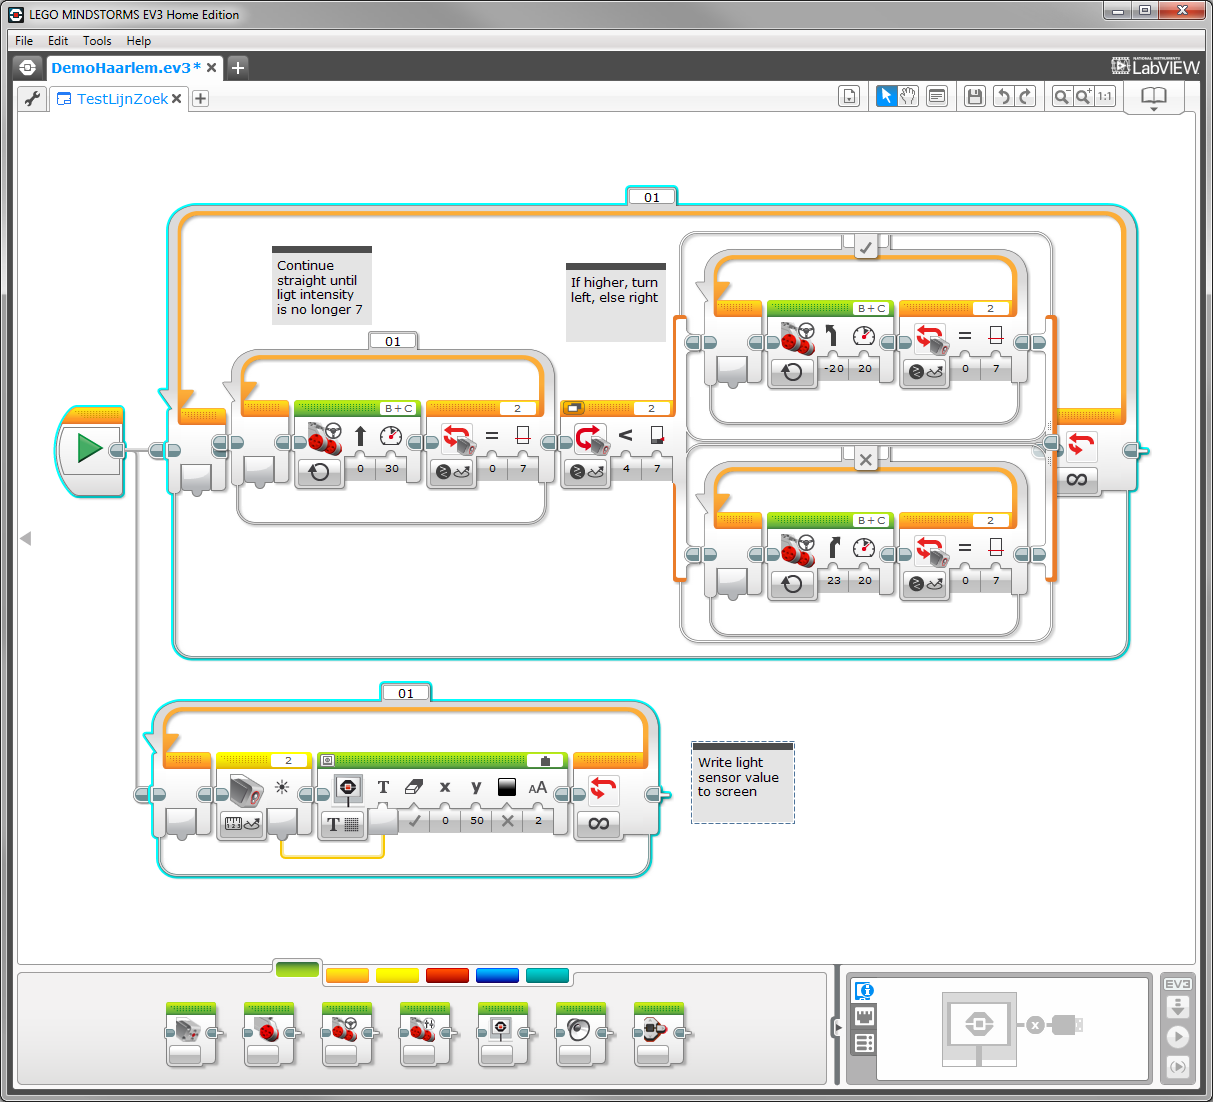
\includegraphics[width=7cm]{img/ms}
\label{fig:ms}
\end{figure}

\subsection{Education Languages}

Many languages have been developed with computer science education in mind (e.g., Scratch~\cite{scratch}, Alice~\cite{aliceIntro}, Kodu~\cite{kodugrammar}, \ms~\cite{lego}), and each language has its own unique structures, abstractions, and programming environment. One advantage of
educational languages, from the user's perspective, is that syntax errors are often prevented, allowing the user to concentrate on program design and logic. For example, the blocks in Scratch and \ms~fit together like building blocks and the selection menu for choosing programming tiles in Kodu dynamically updates based on context. In addition to support to make programming easy, these languages also offer abstractions in the form of objects and subroutines, allowing programmers to create complex code~\cite{Stolee:2011:ECS:1953163.1953197}. As such, these languages, like professional languages, are susceptible to poor design and code smells. In this work, we focus on \ms~and Kodu. 
\todo{Why? Can we justify why these languages, other than convenience?}


\subsubsection{\ms}
\label{sec:lego}
EV3 is the third iteration of the LEGO MINDSTORMS robotics line. It consists of a number of sensors, four motors and an ARM 9 ``intelligent brick''. The robotics kit comes with a control software package, which allows for visual programming of the brick, based on LabView\footnote{\url{http://www.ni.com/labview/}}. The software supports several basic constructs common to programming, including loops and conditionals, as well as more advanced features like parallel execution. Figure \ref{fig:ms} shows the user interface of the EV3 software with a program that makes a robot follow a black line by steering left if the sensor value is below the threshold of 7 and right if the value is above, and in parallel writes the sensor value to the screen. This program demonstrates some of the basic EV3 programming concepts including parallel execution, loops and switches. Blocks have to be connected to the `Play button' on the left with wires to be executed, the block on the lower right is not connected and thus colored gray to indicate this to the user.

In addition to the programming concepts described above, users have the possibility to define `\mbs' which are basically  subroutines. \mbs~may have up to 9 different input parameters and one output parameter. \mbs~cannot be programmed from scratch; they can only be created by selecting blocks in an existing program and clicking `my block builder'. This puts the selected blocks in a new \mb~and replaces the blocks with a call to the newly created \mb, an abstraction action very functionally similar to `extract method' present in most modern IDEs. 

\begin{figure} [tb]
\caption{Two blocks representing the same functionality, one in a regular block and one using a call to a \mb.}
\centering
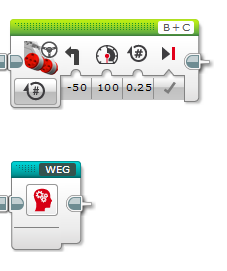
\includegraphics[width=7cm]{img/weg}
\label{fig:weg}
\end{figure}

\begin{figure}[tb]
\caption{The interface of Kodu~showing programming behavior for a bot that moves towards a red apple and then eats it.}
\centering
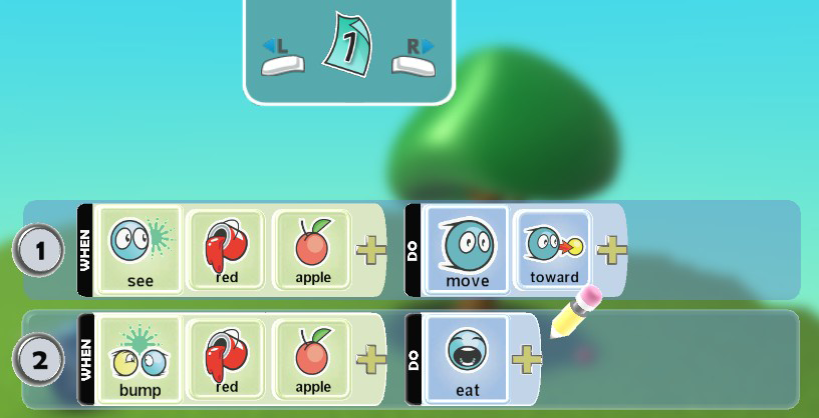
\includegraphics[width=7cm]{img/programmingui.png}
\label{fig:Kodu}
\end{figure}

\subsubsection{Kodu}
Microsoft Research's Kodu is a visual programming language~\cite{kodugrammar} and environment that allows users to create, play, and share their own video games. 
It is available for download on the Xbox and PC and is heavily inspired by robotics, as illustrated by the context of programming in it and its language. 


Users create a world (e.g., land, water, clouds),  add characters and objects, and then can program each character or object (e.g., a kodu robot character, a turtle character, an apple object, a tree object; we use character and object interchangeably) individually. Variables are introduced as scores or properties of characters. Scores are integers and global variables, identified by color or letter, and readable and editable by all characters and objects. Character properties, such as color, glow color, expression and health, are like local variables. A character or object can read and write any of these properties for itself, and it can also read and write selected properties of other objects. 

The programming defines how a character or object can interact with the world, treating each character or object as an autonomous agent. Each object has 12 pages that can be programmed, analogous to methods in an OO language, where the current page defines the current behavior of the object. 
The object's behavior can change by switching between pages to modify state and control flow. 
Each page contains a set of rules, and each rule is in the form of a condition and an action, which form a {\tt when~--~do} clause. The {\tt when} is defined by a sensor (e.g., see, hear, gamepad input) and filters (e.g., apple, gamepad A button). The {\tt do} is defined by an actuator (e.g., movement, shoot) and modifiers (e.g., missile, toward). All the rules on a page are evaluated in a single frame, from top to bottom. 
Despite its unique language, Kodu  can be used to express many basic concepts in computer science, such as variables, boolean logic and conditional control flow~\cite{Stolee:2011:ECS:1953163.1953197}. 

Figure~\ref{fig:Kodu} shows a page and two rules  in Kodu. For the first rule, the condition is, {\tt when see red apple}, and the action is, {\tt move toward it}. The action defines the behavior of this particular character when it sees a red apple, that is, it moves toward it. Since the condition identifies an object (i.e., apple), it becomes the default selector, even though it is not explicitly specified. The second rule, {\tt when bump red apple, do eat}, has a similar condition with a different sensor, {\tt bump}. The action of the second rule, {\tt eat}, indicates that the character should eat any red apple it bumps. 
The programming in Figure~\ref{fig:Kodu} applies to the first page in this character's programming, as indicated by the number one at the top of the screen. The first page is the  start page.

To form more complex boolean logic, rules can also be indented to create complex {\tt when} clauses, where both conditions need to be true for the action to occur. Alternatively, indenting a rule and removing the {\tt when} means that multiple {\tt do} clauses occur for the same trigger condition. 

%\subsubsection{Other Domains}
%End-user programming domains extend beyond spreadsheets and web mashupss. Stolee and Elbaum explore future opportunities for refactoring in educational programming languages~\cite{StoleeTSE2013}. \todo{revisit, this is a bit strange now this paper talks about education too}

%Other end-user programming domains that could benefit from smell analysis and refactoring are mathematical environments like MATLAB, Sage, and Mathematica.

%In particular, the smells related to duplication and poor construction like \emph{long method}, \emph{Many Parameters} and \emph{Dead Code} are prevalent in the four domains studied.
%These smells -- and their respective refactorings -- likely exist in other end-user programming domains, and likely hinder the understandability and maintainability of those programs. Worse even, these smells could lead to errors, and thus these smells are worthy of our attention. 

%\subsection{Future Opportunities in Professional Languages}
%In end-user programming languages, it has been shown that code smells impact the understandability of
%source code~\cite{StoleeTSE2013}. Additionally, being presented with code smells can motivate end-user programmers to improve their code~\cite{chambers2013smell}, and smells in spreadsheets have even been known to reveal actual errors~\cite{Hermans2012intra}. These lessons could extend to professional programming languages. but further study is needed. 
% outside of the end-user programming domains. 
%There has been successful in using automating smell detection, for example, during agile development (e.g.,~\cite{Schumacher:2010:BES:1852786.1852797}). Paired with the end-user evidence, a stronger case can be made to integrate automated smell detection in many domains. 

%\todo{Other data flow languages could benefit from \emph{normalize order of operations} to improve understandability (as it does with YP). }


\section{Definitions of Smells}
\label{sec:definition}
In Section~\ref{subsec:eusmells}, we summarized OO-inspired end-user smells from previous work. In both the Excel and the Yahoo! Pipes work, it was found that OO inspired smells were applied to end-user languages. This leads to the question how broadly applicable code smells are to end-user languages. 

We begin by mapping the smells to two education languages.  Given that this is a first look into code smells in education languages, we limit our exploration to the 11 code smells found in other end-user programming languages, \ms~and Kodu. 
As is common in the other approaches, we define a loose mapping of OO concepts to the end-user languages in question.
The thresholds we used for the study to determine when the presence of a pattern is considered smelly, (e.g., how big must a method be to have a \emph{long method} smell?),  are defined in Section~\ref{sec:study}. 



\subsection{Smells in \ms}
In EV3 programming, \emph{\mbs~} consist of a number of blocks, can be called multiple times, and use input and output. As such they resemble methods in source code, modules in Yahoo Pipes and worksheets in spreadsheets. Based on this translation, we investigate whether and how each of the smells in our catalog  apply to EV3 programs.  

\textbf{Dead Code} It is possible for programming blocks to be disconnected, but the interface clearly indicates this as explained above. However, unused \mbs~can be present in the project without a warning being issued. This is smelly as it makes the program unnecessarily large.\\
\textbf{Deprecated Interface} This is a smell that does not apply, as, to date, there is only one version of the EV3 software and no blocks have been deprecated.\\
\textbf{Duplicate Code} When the same, or very similar combinations of blocks occur, the program suffers from the duplicate code smell.\\
\textbf{Feature envy} While all defined variables within EV3 programs are global, they can be written in a certain \mb~but read in a different one. If, in a given \mb~many variables are read that have been written somewhere else, this is be an occurrence of the feature envy smell. \\
\textbf{Inappropriate Intimacy} Variables can be read in one \mb~but written somewhere else. If there are two \mbs~sharing multiple variables this way, it might be better to combine them.\\
\textbf{Lazy Class} If a \mb~is very small, for example, consisting of just one block, they do not add a lot of value, while impacting understandability, as a user has to navigate to the \mb~to see what its functionality is.\\
\textbf{Long method} If a \mb~grows very large, it will no longer be easy to understand, counteracting the added value of the abstraction.\\
\textbf{Many Parameters} \mbs~can have 9 different parameters, which could be considered too much for easy understandability, especially since parameters need to be connected with wires, potentially leading to visual clutter.\\
\textbf{Message Chain} Since \mbs~can have both input and output parameters, they can form a message chain, in which values are continuously passed until they are used, while they could have been passed directly, outside of the \mbs.\\
\textbf{No-op} It is possible to combine blocks in such a fashion that they do not actually contribute to the functionality of the program. For example, if a user stops the same motor twice, the second stop will be a no-op.\\
\textbf{Unused Field} As explained above, \mbs~can define parameters. However, the user is not forced to use them, hence it is possible to define parameters but not use them.




\subsection{Smells in Kodu}
In Kodu, we consider pages of programming as analogous to methods or classes, similar to how modules are treated in Yahoo!\ Pipes, worksheets in spreadsheets and \mbs~in \ms. \\
\textbf{Dead Code} If there exists a page with programming such that there is no explicit path of control flow from Page~1 to it, it is unreachable and therefore dead. \\
\textbf{Deprecated Interface} Some language features may exist in early versions of Kodu but not be available in future versions. As none of these features were ever deployed, this smell is not possible. \\
\textbf{Duplicate Code} Two pages for the same character with exactly the same set of rules, or two identical rules on a page constitute duplicate code. Alternatively, two rules on the same page with the same {\tt when} clauses (i.e., sensor and filter) but different actions could be consolidated using the indent feature and thus are smelly. \\
\textbf{Feature envy} All global variables, such as game scores, can be read and written by any character. If a certain character reads variables that have been written by another character, this could be an instance of the feature envy smell. \\
\textbf{Inappropriate Intimacy} A character has four local properties that describe its state: color, glow color, expressions (angry, crazy, happy), and health.  If one character frequently checks the properties of another character, this could constitute inappropriate intimacy. \\
\textbf{Lazy Class} If a character has no programming, it could be an instance of the lazy smell. \\
%Characters with no programming are different than objects. Characters can have movement whereas objects cannot. 
\textbf{Long method} A page with many, many rules may be difficult to understand. Some programming could potentially move to other characters.\\ %We counted long methods as those with ten or more rules. 
\textbf{Many Parameters} A game can have 37 different global scores. Games that use many of these could be unnecessarily smelly. \\%We set the threshold at three. 
\textbf{Message Chain} It is possible for a character to create a chain of switches between pages without any logic on the page other than the jump. This would create a long and unnecessary message chain. \\
\textbf{No-op} Jumping to a page with no logic is the logical equivalent of a null pointer. While no error would be raised, the character would no longer have any behavior and would be stuck. Alternatively, rules with {\tt when} clauses but no {\tt do} clauses do not perform any actions. \\
\textbf{Unused Field} A global variable that is written to but not read is an instance of the the unused field smell. \\



\section{Study}
\label{sec:study}
The aim of this paper is to explore the following research question: \textbf{To what extent do code smells occur in programming languages aimed at education?} 
%We divide this question into two subquestions:
%
%\begin{enumerate}
%%\item{How can we define code smells in \ms~and Kodu?}
%\item{How often do the defined code smells occur in \ms~and Kodu?}
%\item{Are there domain specific, non-OO-inspired in \ms~and Kodu?}
%\end{enumerate}
To answer this research question, we analyze and count code smells in programs created in two new domains: a data-flow educational language for programming robots, \ms~software,  and an event-driven educational language for building and playing video games, Kodu. 
In this section, we describe the artifacts and analysis used for the study. 

\subsection{Artifacts}
For each language, we sought to explore programs created by two communities, kids (the intended audience of the languages) and the community at large, which often includes kids and adults. 

\subsubsection{\ms}
We  gathered 17 programs from two data sources. The first source is a weekly robotics club for children aged 8 to 13. The programs collected were designed to participate in two robot competitions: 

A sumo wresting game in which robot have to push each other out of a ring\footnote{\url{http://www.sugobot.com/}}, and a search and rescue game in which robots have to detect a soda can\footnote{\url{http://rcj.robocup.org/rescue.html}}. To obtain a more diverse set of EV3 programs, we also solicited members of the EV3 programming group on Facebook to share their programs with us\footnote{\url{https://www.facebook.com/groups/legomindstorms/permalink/527560164058881/}} and refer to these as programs from the \emph{community}. Nine programs come from this second source. 


\subsubsection{Kodu}
We gathered 27  programs from two data sources. 
For the first data source, we ran a workshop at the Microsoft FUSE lab that introduced children to Kodu Game Lab in a series of three 3-hour sessions.  To recruit participants, we advertised the Kodu workshop using a mailing list of parents interested in Kodu.  
Children between the ages of 9 and 12 volunteered to participate, with parental consent. We collected 17 programs created during the workshop for analysis. 
For the second data source, we randomly sampled 10 programs from the public Xbox Live community. No demographic information was collected about the users. 



\subsection{Analysis}
At a high level, EV3 is a robotics language and Kodu is inspired by robotics. As such, they share some high-level concepts, such as performing actions based on sensor values. This allows us to similarly tune the smell detection thresholds in our studies.

\subsubsection{\ms}
To count the number of instances of the \emph{long method}, a smell was counted when the \mb~had 10 or more blocks, as this is typically the size that all blocks would not fit on the screen anymore. For the \emph{lazy class} we defined smelly as three blocks or fewer. For the  \emph{many parameters} smell, the use of four or more input values as typically in the programs one or two were used.

\subsubsection{Kodu}
%The programs were analyzed  by one of the authors. %Table~\ref{tab:koduanalysis} presents the 17 programs created by children (K1 \dots K17), 10 programs created by the Xbox Live community (K18 \dots K27), and the smells found in each. The \emph{Characters} row defines how many characters and objects are in the program, \emph{Pages} defines how many pages of programming are used by the characters, \emph{Rules} counts all the rules on all the pages, and \emph{HCI Actors} counts the number of characters in the program that are controllable by the Xbox controller, mouse, or keyboard. 
To count the number of instances of the \emph{long method}, a smell was counted when the page had 10 or more rules. For the  \emph{many parameters} smell, the use of four or more game scores. These thresholds were determined by the authors as 10 rules cannot be viewed on a screen screen without scrolling and only a couple games used more than three game scores; these are the same as those used for EV3. 


\section{Results}
\label{sec:results}
Results for the smell detection analysis in \ms~and Kodu are presented here. When investigating the programs in both languages, we found that they indeed can suffer from OO-inspired smells. 

%Table \ref{tab:robotica} shows an overview of the EV3 programs from the Sumo (L1...L5), RoboCup (L6...L8) and community (L9...L17) programs and the smells found in them. The EV3 programming interface divides the programming blocks into 6 categories, indicated in the colored tabs in Figure \ref{fig:ms}. The number of blocks in each of the categories for the programs are listed in the first 6 rows in Table \ref{tab:robotica}. Furthermore we have counted the number of comment blocks: special blocks that do not perform any action but are used to document programs, the number of variables: blocks that store a value that can be retrieved later, and the number of \mbs~ created in the program. The \emph{Total Blocks} column provides an indication of program size.  


\subsection{\ms}
On average, the programs from children's robotics club had 2.5 smells each and the programs from the community  had 1.4 smells each, though  the people submitting through the Facebook community most likely sent in nicely polished programs. Furthermore, the community programs were generally smaller (a median of 17 versus 23 total blocks) exhibiting more reuse as they more often used call to \mbs. There are only three smells that do not occur in any of the programs: \emph{deprecated interface} (not applicable), \emph{inappropriate intimacy} and \emph{message chain}.

Next, we discuss the three most common smells within the EV3 programs. 
%Duplicate Code occurs most, in over half of the programs. 

%\begin{figure} [ht]
%\caption{The project properties screen for program L1, showing the three \mbs, but not indicating which are used.}
%\centering
%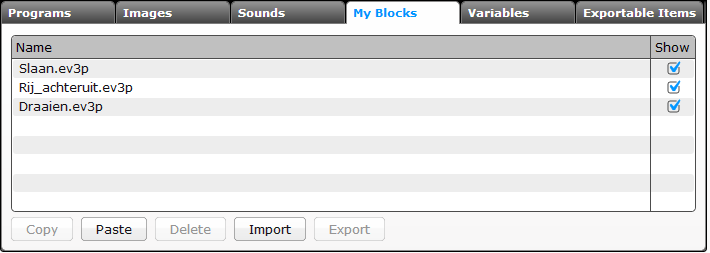
\includegraphics[width=\columnwidth]{img/overview-small}
%\label{fig:overview}
%\end{figure}

\paragraph{Duplicate Code}
The most common smell we found in the programs is the \emph{duplicate code} smell, which 65\% of the programs suffer from. Duplication comes in various forms.  Some of the programs use two motor blocks in a row, which could have been merged. For example, consider the two blocks from program L17, shown in Figure \ref{fig:dup_ev3}. This might have been challenging for the users to detect, as they use two slight variations of the motor block, but the two behave exactly the same in this case. Hence, one block moving forward 1.25 would have sufficed. Other programs exhibit duplication at a high level, such as the two \mbs~in program L16, depicted in Figure \ref{fig:dup_ev3_myblocks}. Here, the two \mbs~perform the exact same operation, but on a different motor. By connecting the name of the motor to a parameter, like angle and speed already are, the same functionality could have been implemented with one \mb.

\begin{figure} [tb]
\caption{The duplication smell in two subsequent motor blocks. Since both have the same power and direction, they could have been merged. }
\centering
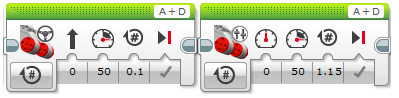
\includegraphics[width=6cm]{img/dup_ev3}
\label{fig:dup_ev3}
\end{figure}

\begin{figure} [tb]
\caption{The duplication smell in two different but very similar \mbs. By parameterizing the motor name, this could have been implemented with 1 \mb. }
\centering
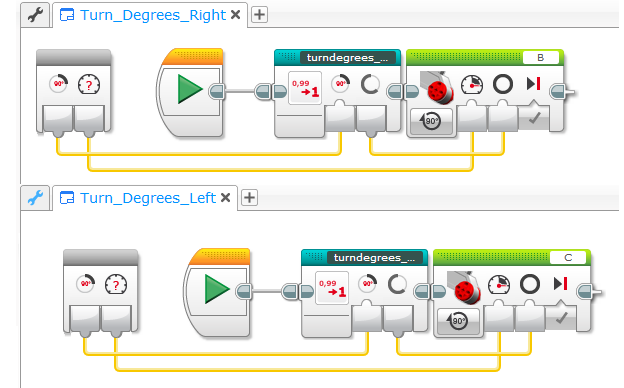
\includegraphics[width=6cm]{img/dup_ev3_myblocks}
\label{fig:dup_ev3_myblocks}
\end{figure}

\paragraph{Dead Code}
The second most common smell is \emph{dead code}. In 41\% of the programs we found \mbs~that no longer connected to one of programs. This can pose a problem, firstly, for understandability, but also poses a practical program as the EV3 environment compiles and transfers all programs and \mbs~to the physical brick, so dead code takes up unnecessary space on the brick. The \emph{dead code} smells is more common in the robotics class programs than in the community programs. This is to be expected, as users felt confident enough to share their programs, so probably they either programs before sharing them, or selected `clean' programs to share.

Looking at the EV3 programming interface, it is not that surprising that users forget about disconnected \mbs, as the EV3 interface provided no information on which \mb~is used and where. Even worse, users can delete \mbs~that are still being called, without a warning being issued about this. After removal of a \mb~ in use, the program no longer compiles.

%If we look at the project properties screen, shown in Figure \ref{fig:overview}, one can see that there is no information about which \mb~is used, and where. 
%Even worse, users can delete \mbs~that are still being called, without a warning being issued about this. After removal of a \mb~ in use, the program no longer compiles.


\paragraph{Lazy Class}
A \emph{lazy class}, which we count as \mbs~containing three or fewer blocks, are also relatively common, occurring in four of the programs. However, we only find this smell in the programs from the robotics club and not in the community programs. Many `lazy \mbs'~were relatively small, consisting of two or three blocks, or even one in some cases. In general, small abstraction are considered smelly, as understanding the abstraction requires inspecting it, which might not be worth it for small classes, methods or \mbs. However, for EV3 this smell might not be as smelly as in other languages, as the programming interface does not allow regular blocks to be named, but it does allow this for \mbs. So by making a \mb, users can express the intent of a coherent set of blocks, even if this set consist of just one block. 

As an example, consider the two blocks from program L6, shown in Figure \ref{fig:weg}. The left block is regular block controlling a motor, while the right one is a call to a \mb~with the same functionality. The first one just expresses what the robot must do, but the second one expresses the intent (`weg' meaning flee). Using the \mb~here serves as an alternative for adding comment blocks. While small \mbs~still add overhead, as the user need to navigate to the block to understand it, the trade off might be different for EV3 than in other languages.

%\paragraph{Long method}
%Long method occurs in four programs, but, contrary to Lazy Class, is found mostly in the Facebook programs. This is to be expected, as more experienced users can handle bigger \mbs, while the kids from the robotics club stick with making small blocks.

\subsubsection{Summary}
To summarize, smells indeed occur in the EV3 programs. Smells are found in 88\% of the programs, with \emph{duplicate code}, \emph{dead code} and \emph{lazy class} (small abstractions) observed most often. Hence we conclude that smells from OO are applicable to this end-user language, though for the \emph{lazy class} smell, the impact might be different in the context of EV3. 


\subsection{Kodu}
On average, the programs from children had 2.3 smells each and the programs from the community had 3.5 smells each, though we note that the programs from the community tend to be larger (e.g., an average of 101 rules vs. 42 rules). Next, we discuss the three most common smells found in the Kodu programs, appearing in 40\% or more of the sample. The remaining smells appear in 25\% or fewer programs. 

\subsubsection{Lazy class}
The \emph{lazy class} smell was the most common, appearing in 79\% of the Kodu programs. This smell is intended to capture when a character is placed in the world but has no programming, and thus no behavior. In some cases, this may not be a smell at all, such as when characters are used as decorations in the world (e.g., trees and rocks). In others, it could be similar to an object that is created but that has no behavior. 

\subsubsection{Duplicate Code}
This smell was present in 61\% of the programs. All instances were that of duplicate {\tt when} clauses within a page, and there were no instances of identical rules on a page or identical pages within the same character. The prevalence of this smell shows a missed opportunity for consolidating the code. 

\subsubsection{No-op}
The next most-common smell is the no-op, present in 41\% of the programs. All instances of this smell were rules without {\tt do} clauses, rather than jumping to pages without logic.  This is probably the product of the rapid cycling between testing and developing observed in Kodu development~\cite{Stolee:2011:ECS:1953163.1953197}; since the clauses have no actionable logic, keeping them in the code does not impact the semantics of the program, though it may impact performance. We note that none of the rules following these no-op clauses were indented to create a conditional conjunction. 


\subsubsection{Summary}
To summarize, smells indeed occur in the Kodu programs. Smells are found in 93\% of the programs, with \emph{lazy class}, \emph{duplicate code},  and \emph{no-op} (small abstractions) appearing most often. Hence we conclude that smells from OO are applicable to this end-user language. 

\subsection{Summary}
Table~\ref{tab:smellsummary} summarizes the frequencies of occurrence of the various smells in the EV3 and Kodu programs. Overall, 88\% of the EV3 and 93\% of the Kodu programs contained at least one smell. Coupled with the 81\% of Yahoo!\ Pipes programs~\cite{StoleeTSE2013} and 42\% of Excel programs~\cite{Hermans2012intra} that were previously found to be smelly, this provides further evidence of the prevalence of smells in end-user programs. 

As with code written by other end-user programmers~\cite{StoleeTSE2013}, \emph{duplicate code} is prevalent in EV3 and Kodu programs, affecting over 60\% of the samples in both languages. The other two smells that were studied in Excel and Yahoo!\ Pipes, \emph{lazy class} and \emph{long method}, are present in at least 24\% of the studied EV3 and Kodu programs, illustrating commonality across all end-user programming domains. 

\emph{Dead code} is more frequently found in EV3 and \emph{lazy class} smells are more common in Kodu. The \emph{no-op} smell is present in 41\% of the Kodu programs, which is similar in spirit to the 41\% of EV3 programs with \emph{dead code}. \emph{Feature envy} was also prevalent across both languages, appearing in 18\% and 22\% of the EV3 and Kodu programs, respectively. 
We observe that the occurring smells seem to be anti-patterns that occur in programming in general, independent of the programming language. 

\begin{table}
\caption{Summary of Smells Across EV3 and Kodu Programs \label{tab:smellsummary}}
\begin{small}
\begin{center}
\begin{tabular}{l | r r}
&EV3&Kodu\\ \hline
Dead Code&41\%&11\%\\
Deprecated Interfaces & 0\% & 0\%\\
Duplicate Code&65\%&61\%\\
Feature Envy&18\%&22\%\\
Inappropriate Intimacy&0\%&4\%\\
Lazy Class&24\%&79\%\\
Long method&24\%&25\%\\
Many Parameters&6\%&4\%\\
Message Chain&0\%&4\%\\
No-op&12\%&41\%\\
Unused Field&12\%&25\%\\ \hline
Any smell & 88\% & 93\%
\end{tabular}
\end{center}
\end{small}
\end{table}


\section{Beyond OO Smells}
\label{sec:beyond}

\label{sec:background:domain}
In the previous sections we have looked at OO smells in end-user programming languages. However, end-user programming environments offer many opportunities to define smells based on user behavior or unique elements of the domain. Hence in this section we explore opportunities for new smells in end-user domains that extend beyond the OO-inspired smells in Section~\ref{sec:background}. 

\subsection{End-User Programming Smells}
\label{sec:eupsmells}
%Many smells beyond the OO language exist in several of the domains studied. 
The following smells appear in at least two  end-user programming languages but are not related to OO smells. 

\subsubsection{Layout smells}
The EV3 and Yahoo!\ Pipes languages are visual and involve connecting boxes with wires, making it easy to create an unwieldily structure. EV3 is especially problematic as it lacks an auto-layouting function.

A special case where layout issues arise is when a user creates a \mb. Remember that \mbs~can only be created with an `extract method' operation. If this operation is called, all selected are moved to the newly created \mb, and are replaced by one block that is a call to this new \mb. Other than that, the layout remains unchanged. So if a big \mb~is created, the program will now have a big gap, making the program harder to read. This, and other layout smells too are unique to visual languages and can impede understandability. 

%Katie just realized this is true of ALL LANGUAGES EVERYWHERE, since most don't fit on whatever screen. Oops. 
%\subsubsection{Lack of Visual Abstraction smell}
%Visual languages can suffer from a visual lack of abstraction smell when the entire program does not fit well on the screen and thus is difficult to comprehend. The threshold for the presence of this smell is clearly dependent on screen size, but nonetheless, it can have an impact on program maintainability~\cite{StoleeTSE2013}. 
%
%This is similar to the \emph{long method} smell in Kodu and EV3, the \emph{duplicate code} smell in Yahoo Pipes (named \emph{isomorphic paths}), or \emph{many operations} in Excel.
%	
%One way to deal with this kind of visual smell is through abstraction. The Yahoo Pipes language provides this through the subpipe module, EV3 through MyBlocks, and Excel through worksheets.  Including subpages or being able to collapse rules on a page would facilitate this in Kodu but support for that is currently not available. 


%\subsubsection{Lack of Comments smell} \todo{I do not think this is a very strong `smell', I'd propose to drop it}
%The lack of comments in a program can make it difficult to understand. Kodu and Yahoo Pipes both do not have a commenting feature in the programming language and development environment, often making it difficult to understand another's work or maintain old code. 

\subsubsection{Programming Organization smell}
Communities of programmers often have standards for how to structure program code. These \emph{population-based} smells were first introduced for Yahoo Pipes~\cite{StoleeTSE2013} and can be uncovered by exploring programs written by the community. In Kodu, often the rules that map a character's behavior to user input from a gamepad, keyboard or mouse are at the top of a page and the remaining logic is at the bottom. Deviating from this structure can lead to programs that are more difficult to understand when shared. In spreadsheets, there have been attempts to define programming standards\footnote{\url{www.fast-standard.org/}}, if such a standard is common within a company, a deviation could be considered smelly as well.


\paragraph{Conflicting Outcomes smell}
In robotics inspired languages, actions are performed based on sensor values. This is true of EV3 and Kodu and  provides the opportunity to create conflicting outcomes for the same sensor. 
In Kodu, this can happen when the same \texttt{when} clause is followed by conflicting \texttt{do} clauses. For example, consider the following two Kodu rules:
\begin{verbatim}
(1) When hear turtle : do score 1 red
(2) When hear turtle : do unscore 1 red
\end{verbatim}
\noindent The {\tt do} clauses are in conflict, both scoring and unscoring the red variable score by 1. In if the {\tt do} clause on rule~2 was instead, {\tt do score 1 red}, then the rules would both execute outcome would be adding 2 to the red score. 
In EV3, the same situation can occur, as it supports \texttt{wait} blocks, which are very similar to a \texttt{when} clause. For example, a user can define a \texttt{wait} block for a sensor to detect black. Only when the \texttt{wait} block returns true the following block is executed. Similar to Kodu, when to similar \texttt{wait} blocks would be defined with conflicting following blocks, for example one where the motor moves 60 degrees clockwise and one where it moves 60 degrees counterclockwise, they would cancel each other out too.

Flagging conflicting rules during development would help alert users to this smell. 

\subsection{Domain-Specific Smells}
Each end-user domain has unique characteristics that create opportunities for defining domain-specific smells. In Yahoo Pipes, prior work has explored the presence of broken or deprecated data sources as a smell unique to the domain~\cite{StoleeTSE2013}. In Excel, prior work defined referring to an empty cells are smelly~\cite{cunha2012towards}. Here, we explore smells in EV3 and Kodu that are unique to their languages and environments. 

\subsubsection{EV3}
%\subsubsection{Hardware/Software Interface Smells}
The \ms~programming language differs significantly from the other end-user domains, as EV3 programmers work with both software and hardware. While programming, users need to configure motor blocks to the right port, for example the blocks in Figure \ref{fig:dup_ev3} are controlling motors A and D. This means that, when a user has the wrong mental model of what motor is connected to what port, the program will not function as wanted. It appears users run into this issue too, some of the programs contained comment blocks in which the mapping was described, in an effort to ensure proper mapping. Hence a smell unique to the EV3 domain is a wrong mapping between the robot in reality and the motor and sensor blocks, forming a \emph{hardware/software interface smell}. 

\subsubsection{Kodu}
The Kodu environment involves designing games, programming games, and playing games. This, paired with the unique event-driven language, creates unique opportunities for domain-specific Kodu smells. 

% 



\paragraph{Single Input Device smell}
Games in Kodu can be programmed and played using an Xbox controller or a keyboard and mouse. Many games are programed assuming a particular device for input, such as an Xbox. However, when playing a game in a different environment, that device may not be available, and thus the game is not portable. This smell could be mitigated by adding analogous rules for other input devices, such as mapping the gamepad trigger switches to the keyboard shift keys or mapping the right stick to movement. 

\paragraph{Lost Character smell}
The \emph{lazy class} smell is related to a non-programmed character or object. Characters and objects need to be clicked on to be programs. A design smell can then manifest when a programmed object cannot be easily found in the world, and thus there is program behavior that is difficult to change. Resolving this smell could involve physically moving the characters or objects to be more accessible, adding a color or speech bubble above them as a marker, or by adding an environment feature that maintains a list of programmed and non-programmed characters that can be accessed. 	

\section{Related Work}

\label{sec:related_work}
Related to the current research are efforts on code smells within traditional languages, we start with the work of Fowler\cite{Fowl1999}. His book gives an overview of code smells and corresponding refactorings. Recent efforts focused on the automatic identification of code smells by means of metrics. Marinescu~\cite{Mari2001} for instance, uses metrics to identify \emph{suspect} classes, those classes that might have design flaws. 
%Lanza and Marinescu~\cite{Lanz06} explain this methodology in more detail. Alves \emph{et al.}~\cite{Alves2010} focus on a strategy to obtain thresholds for metrics from a benchmark. Olbrich \emph{et al.} furthermore investigates the changes in smells over time, and discusses their impact~\cite{Olbr2009}.

Within end-user programming, this paper builds upon two lines of related work. First, the work of Stolee and Elbaum that studied smells~\cite{StoleeTSE2013} and refactorings~\cite{Stolee2011}. They designed a number of smells by transforming known OO smells to the domain of Yahoo Pipes. The second direction is the work by Hermans \emph{et al.} that also took OO smells as an inspiration for a number of smells in spreadsheets~\cite{Hermans2012intra, Hermans2012inter}. Subsequently they described corresponding refactorings~\cite{Hermans2012intraExt} and a tool that applies refactorings~\cite{hermans2014bumblebee}. This final work generalized previous work by Badame and Dig~\cite{badame2012refactoring}.

%In end-user programming environments, user input and logic are often more closely linked than they are in general purpose languages, and as such analyzing the input data as opposed to the logic can also be used as a means of \emph{smell detection}. This is a direction that has been applied to spreadsheets. Cunha et. al \cite{cunha2012towards} for example look at anomalies in the data and define these as smells. Examples of this are \textit{Standard Deviation} which occurs if one assumes a normal distribution for a column in numeric values and the column contains values which fall outside two standard deviations. In more recent work, Barowy et. Al \cite{barowy2014checkcell} take a more formalized approach which they label ``Data Debugging''. Their solution uses statistical analysis to find values with an unusually high impact on the calculated results in a spreadsheet, as such values are likely either very important or erroneous.

In addition two above described work on Yahoo Pipes and spreadsheets, there is previous smells work on other end-user environments too, like performance smells in LabView, a visual language for system-design~\cite{chambers2013smell, chambers2015impact}. 

Research related to  EV3 and Kodu predominantly explores 
language design~\cite{Fristoe:2011:SSE:2159365.2159396, Stolee:2011:ECS:1953163.1953197, MacLaurin:2009:KEP:1536513.1536516, MacLaurin:2011:DKT:1925844.1926413} 
and educational benefits~\cite{Fowler:2011:KGL:2159365.2159398, Touretzky:2013:AKC:2445196.2445374, Barnes:2002:TIJ:563340.563397, Hood:2005:TPL:1067445.1067454}. 
%The language of Kodu can be used to express computer science concepts commonly taught in introductory classes, such as boolean logic, variables, and objects~\cite{Stolee:2011:ECS:1953163.1953197}. 
There is some, albeit limited, work on detecting code smells in educational languages. Chatley and Timbul describe Kenya, a simple programming language for educational purposes, which they have integrated into the Eclipse environment~\cite{Chatley2005}. They built features that allow the detection of `bad style' in programs to be detected and reported as code is written, concentrating on encouraging students to program like they were taught in class. This work might indicate that smell detection can be useful for education, but the authors  did notevaluate the usefulness of this approach.


%\section{Discussion}
%\label{sec:discussion}
%
%Based on the research and results for smell detection in end-user programming domains, there are many directions for future work in the domains studied and other end-user domains.
%
%



\section{Threats to Validity}
\label{sec:threats}
The threats to validity of this work inherit the threats to validity of the original studies~\cite{Stolee2015, Stolee2011, StoleeTSE2013, Hermans2011, Hermans2012intra, Hermans2012inter} on end-user smells in spreadsheets and Yahoo Pipes.

%Three domains studied in this paper are dataflow languages, and the smells and refactorings may not generalize to other end-user programming domains. However, we mitigate this threat by analyzing Kodu, an event-driven language, and show that the smells are also applicable in that context. This provides more evidence of the generality of these smells. 

We have defined OO smells in two languages, EV3~and Kodu, yet we have not evaluated whether these smells matter to the end users. Future work is needed to determine the impact of these smell on users of the languages. 

In Kodu, the presence of the \emph{lazy class} smell may be intentional and simply represent a design decision (i.e., a rock is not programmed because it is there purely for aesthetics), and in EV3 the this smell might occur because users make up for the lack of ability to name single blocks. Evaluating these smells with actual users will help tease out when code is smelly and when it is actually designed intentionally. 

We have sampled programs from two sources for each EV3 and Kodu, yet these programs may not be representative of what children and community members create. A larger-scale analysis is necessary to generalize these findings to the populations of EV3 and Kodu programs. 

\section{Conclusion}
\label{sec:conclusions}
This paper describes code smells for two new end- user programming domain, not yet studied in the context of code smells: \ms~and Kodu. We present an evaluation of these code smells in the form of two case studies. The results show that indeed many of the catalog's smells apply in the new domains, and \emph{lazy class} (small abstractions), \emph{duplicate code} and \emph{dead code} occur frequently in these educational languages. The contributions of this paper are:

\begin{itemize} \itemsep -0.25pt
	\item A definition of end-user programming smells in \ms~and Kodu each domain (Section \ref{sec:definition})
	\item Two case studies investigating end-user smells in educational programming languages: \ms~and Kodu each domain  (Section \ref{sec:study})
	\item Identification of future opportunities for domain-specific, non-OO-inspired smell detection in end-user programming domains (Section \ref {sec:beyond})
\end{itemize}

In the end, we observe that the original concept of code smells is applicable to end-user languages, of a quite different character than the textual languages aimed at professional developers that the smells were originally defined for. This underlines the applicability of these smells, and also warrants further research into issues end-users encounter while programming. For example, exploring the impact of code smells on children who use the educational languages or designing user-friendly refactoring tools for visual languages are potential future directions. 
Furthermore, studying the smells in a fresh context provides new insight on how to use smells in software engineering and could even give rise to new types of smells. 

\balance

\section*{Acknowledgements}
Special thanks to Stephen Coy for his help with Kodu, to all kids at `Instituut het Centrum' and the members of Facebook group `legomindstorms' for sharing their programs. This work is supported in part by  NSF SHF-EAGER-1446932 and the Harpole-Pentair endowment at Iowa State University.


\bibliographystyle{IEEEtran}
\bibliography{literaturelist}

\end{document}